\chapter{How I Turned \$50{,}000 Into \$20 Billion}

This chapter should be read as companion notes to an interview rather than as a textbook chapter that merely borrows a few business facts. The lecture opens with spectacle, narrows immediately to origin, and only then begins to unfold its arithmetic. We start with the puzzle of immense wealth built on a narrow product, pass through rejection and first funding, then move into leverage, scale, ownership, and finally the thin-margin logic that returns the whole story to the table. No validated screenshots survived curation for this lecture, so every figure below is a transcript-derived reconstruction rather than a transcription of visible board work.

\section{The Billionaire Chicken-Finger Paradox}

The lecture begins by setting a trap for our intuition. We are first told that we are about to meet one of the richest men in the world, and then the answer to the question of origin comes back in language almost absurdly plain: he sells chicken fingers. That compression is not decorative. It is the first real problem the lecture gives us.

The host then does something structurally important. He flies to Baton Rouge, to the original Raising Cane's location, and he insists on beginning at the ``mothership.'' The first store is not scenery. It is the initial condition from which the later business must be measured. The same opening sequence also stresses that this is, for the host, an unusual billionaire route. He had interviewed billionaires across many sectors, but not one whose fortune had been built through fast-food repetition of such a narrow product.

The lecture places three scale markers on the table early:
\begin{equation}
W > \$20\,\text{billion},\qquad N>900,\qquad Y_{\max}\approx \$400\,\text{million}.
\end{equation}
Here \(W\) denotes reported net worth, \(N\) the number of locations, and \(Y_{\max}\) the reported best single-year earnings figure cited in the interview. These numbers do not yet explain anything. They tell us only that the machine whose origin we are about to study is very large.

What matters for the notes is the order. First the lecture creates astonishment. Then it relocates us to the original store. Only then does it ask how the machine was built.

\section{Rejection Before Proof}

\paragraph{Anecdote.}
Graves describes a familiar entrepreneurial childhood: lemonade stands, cutting grass for money, and then early work in restaurants. By college he had already formed a clear view of the business he wanted to build. He proposed a restaurant centered on chicken fingers and received the lowest grade in the class. The professor, as Graves recalls it, did not deny that the plan was carefully assembled; he denied that the concept could work. A narrow menu seemed backward at a moment when other chains were broadening menus and signaling variety.

\paragraph{Claim.}
The lecture's first real business claim is therefore not yet about capital or operations. It is about the interval before proof. Rejection at that stage is not yet market evidence; it is prior judgment. That distinction matters because the host immediately widens the point. He does not leave the story in the classroom. He generalizes it to the entrepreneur who is still unknown, still unproven, and still absorbing refusal.

\subsection{Question \& Answer}

\paragraph{Question.}
What do we do with rejection before we have any credibility at all?

\paragraph{Answer.}
Graves's answer is direct: use it as fuel. That answer sounds simple, but its place in the lecture gives it weight. He is not speaking from a position of later prestige. He is describing the period in which the entrepreneur possesses no demonstrated model, no operating numbers, and no authority except his own belief and effort.

\paragraph{Mechanism.}
The mechanism is psychological, but the lecture does not leave it vague. The entrepreneur either lets refusal collapse action, or he converts refusal into additional work. The host reinforces this by invoking his own early experience of repeated rejection while building his media business. The effect is to prepare the next transition: once belief survives rejection, the next obstacle is not social disapproval but the concrete difficulty of funding a capital-intensive first store.

\section{Financing the First Store}

\paragraph{Anecdote.}
The next question arrives exactly where it should. The host asks how one starts a restaurant when restaurants are expensive and banks do not want to lend. Graves answers without romanticizing the difficulty. He says he was turned down by the bankers in town. Because of that, he had to raise money himself, and he describes a period of physically hard work, including commercial fishing in Alaska. The geographical details in the transcript are slightly noisy, so it is best to keep the broad point rather than overstate the itinerary: he went where hard labor could produce cash.

Once enough personal equity existed, Graves says he was able to use SBA-backed lending and other small-business support structures to bridge the remaining gap. The institutions are named somewhat garbled in the transcript, so here too we should keep the structure more than the exact proper nouns.

\paragraph{Claim.}
The lecture's funding logic is staged rather than monolithic:
\begin{align}
K_0 &= E_0 + L_0,\\
E_0 &\approx \$50{,}000,\qquad L_0 \approx \$50{,}000,\\
K_0 &\approx \$100{,}000.
\end{align}
Here \(K_0\) is the deployable capital for the first store, \(E_0\) the founder's self-raised equity, and \(L_0\) the later SBA-backed borrowing.

\begin{figure}[h]
\centering
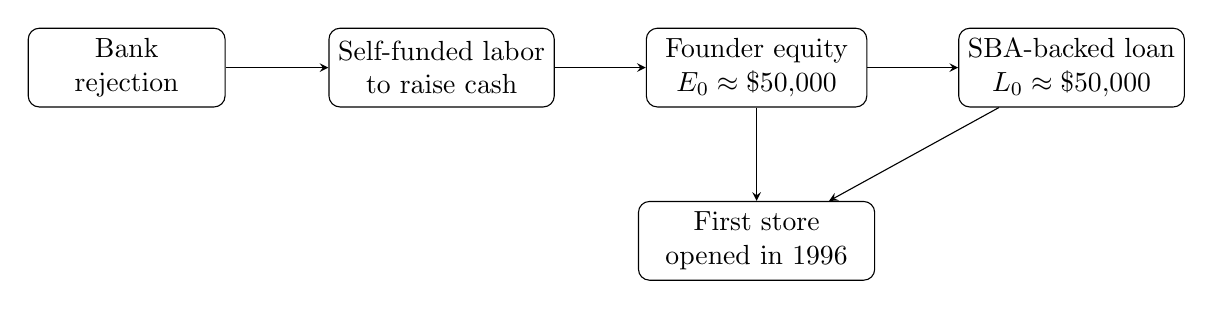
\begin{tikzpicture}[>=stealth]
\node[draw, rounded corners, align=center, minimum width=2.5cm, minimum height=1cm] (a) at (0,0) {Bank\\rejection};
\node[draw, rounded corners, align=center, minimum width=2.8cm, minimum height=1cm] (b) at (4,0) {Self-funded labor\\to raise cash};
\node[draw, rounded corners, align=center, minimum width=2.8cm, minimum height=1cm] (c) at (8,0) {Founder equity\\\(E_0\approx \$50{,}000\)};
\node[draw, rounded corners, align=center, minimum width=2.8cm, minimum height=1cm] (d) at (12,0) {SBA-backed loan\\\(L_0\approx \$50{,}000\)};
\node[draw, rounded corners, align=center, minimum width=3.0cm, minimum height=1cm] (e) at (8,-2.2) {First store\\opened in 1996};

\draw[->] (a) -- (b);
\draw[->] (b) -- (c);
\draw[->] (c) -- (d);
\draw[->] (c) -- (e);
\draw[->] (d) -- (e);
\end{tikzpicture}
\end{figure}

\paragraph{Mechanism.}
What the lecture emphasizes is sequence. We do not begin by demanding that the whole market believe in us. We begin by making ourselves more fundable. Cash raised through labor becomes equity; equity makes a lender's risk smaller; public entrepreneurial infrastructure then becomes usable. The first store is financed not by one magical approval but by a sequence of increasingly credible steps.

\subsection{Question \& Answer}

\paragraph{Question.}
How do we start a capital-intensive business when ordinary banks say no?

\paragraph{Answer.}
We first reduce the size of the question. Instead of asking the bank to finance the entire uncertainty, we finance a portion ourselves, learn enough to speak credibly, and then ask the bank to finance the remaining gap. The lecture's answer is not that capital is easy to find; it is that fundability can be built.

\section{Know the Numbers, Then Negotiate}

Once the first capital stack is in place, the lecture moves from money to argument. The host asks what Graves learned about negotiating with banks, and Graves answers with a structure rather than a slogan: know the numbers inside and out, and think in low, medium, and high cases.

We may write the forecast logic as
\begin{align}
\Pi_{\mathrm{low}} &\approx 0,\\
\Pi_{\mathrm{med}} &> 0,\\
\Pi_{\mathrm{high}} &> \Pi_{\mathrm{med}}.
\end{align}
The low case is the break-even or downside-survival case. The medium case is the ordinary profitable case. The high case is the upside case in which the business produces stronger profits and repays the lender more quickly.

\begin{figure}[h]
\centering
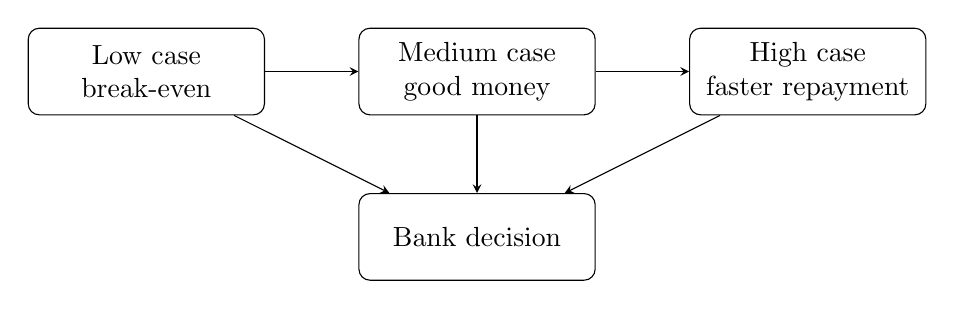
\begin{tikzpicture}[>=stealth]
\node[draw, rounded corners, align=center, minimum width=3cm, minimum height=1.1cm] (l) at (0,0) {Low case\\break-even};
\node[draw, rounded corners, align=center, minimum width=3cm, minimum height=1.1cm] (m) at (4.2,0) {Medium case\\good money};
\node[draw, rounded corners, align=center, minimum width=3cm, minimum height=1.1cm] (h) at (8.4,0) {High case\\faster repayment};
\node[draw, rounded corners, align=center, minimum width=3cm, minimum height=1.1cm] (b) at (4.2,-2.1) {Bank decision};

\draw[->] (l) -- (m);
\draw[->] (m) -- (h);
\draw[->] (m) -- (b);
\draw[->] (l) -- (b);
\draw[->] (h) -- (b);
\end{tikzpicture}
\end{figure}

The lecture's central underwriting intuition is then simple:
\begin{equation}
\Pi_{\mathrm{low}} \ge 0
\quad\Longrightarrow\quad
\text{the business survives even in the downside case.}
\end{equation}
That does not make the business safe in any absolute sense, but it makes the proposal legible. A bank can understand a business that still makes sense when the optimistic scenario fails to arrive.

\paragraph{Worked forecast logic.}
\begin{enumerate}
\item The low case must be hard enough to matter.
\item The medium case must show ordinary economic health, not merely survival.
\item The high case must not be fantasy; it must explain why the lender benefits if execution is unusually strong.
\item If the numbers genuinely work and one lender refuses them, Graves's advice is not to deform the numbers merely to win approval. It is to take the same coherent case to another lender.
\end{enumerate}

This section also contains a formal interruption in the original video. After Graves gives his account of negotiation and before the next major business lesson, the host inserts a long promotional segment about his own network and paid community. In a faithful written chapter we should not pretend that interruption never happened, but neither should we fold it into Graves's doctrine. The clean solution is to bracket it, then return to the interview where the lecture itself returns: the next question is about the best financial advice Graves ever received, and his answer is a near-disaster.

\section{Leverage, Shock, and Scale by Focus}

\paragraph{Anecdote.}
When the interview resumes, Graves does not offer a triumphalist maxim. He says he almost broke the business by overleveraging it while young and growing. Then Hurricane Katrina hit. Between \(21\) and \(28\) restaurants went down, but the banks still had to be paid.

\paragraph{Claim.}
The lecture's anti-fragility point is stark. Growth financed by debt may feel powerful in normal conditions, but a sufficiently large external shock turns fixed obligations into a constraint on survival. The operational base can be written as
\begin{align}
N_{\mathrm{eff}} &= N - N_{\mathrm{down}},\\
N_{\mathrm{down}} &\in [21,28].
\end{align}
Here \(N_{\mathrm{down}}\) is the number of temporarily inoperative restaurants after the storm. If operating capacity falls while bank obligations remain fixed, the business is squeezed.

We do not have a full cash-flow model from the lecture, so we should not invent one. But the direction of stress is perfectly clear:
\begin{equation}
R_{\mathrm{eff}}\downarrow
\qquad \text{while} \qquad
DS \ \text{stays fixed or nearly fixed.}
\end{equation}
Here \(R_{\mathrm{eff}}\) is effective revenue under disruption and \(DS\) is debt service.

\paragraph{Mechanism.}
That is why the lecture's financial correction is not ``stop growing'' but ``grow with more equity.'' Debt is not condemned in the abstract; overleverage is. The founder learns not merely from success but from proximity to failure.

The host then makes the right transition. Having heard that bad growth can be dangerous, he asks how good growth works. Graves's answer is the opposite of menu sprawl. Do one thing and do it better than anyone else. In restaurants, he says, the thing must be craveable.

The scale path is given almost as a visual sequence:
\begin{equation}
N: 1 \longrightarrow 10 \longrightarrow 100 \longrightarrow 900+.
\end{equation}
The lecture's point is that this is not diversification first. It is repetition of a focused operating unit.

\begin{figure}[h]
\centering
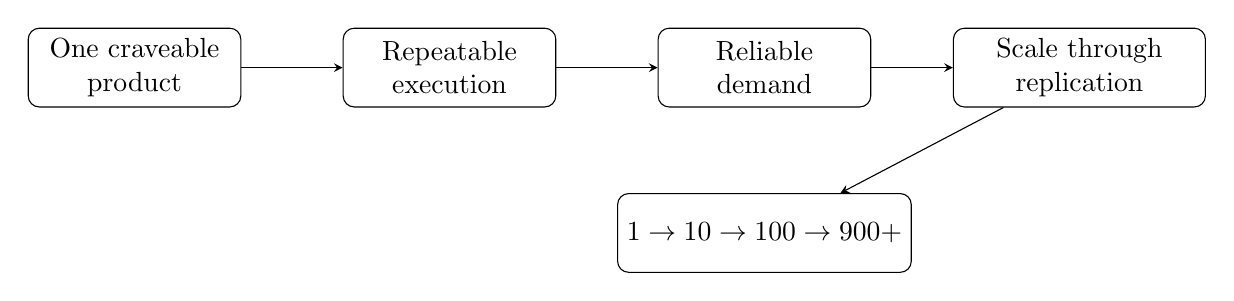
\begin{tikzpicture}[>=stealth]
\node[draw, rounded corners, align=center, minimum width=2.7cm, minimum height=1cm] (a) at (0,0) {One craveable\\product};
\node[draw, rounded corners, align=center, minimum width=2.7cm, minimum height=1cm] (b) at (4,0) {Repeatable\\execution};
\node[draw, rounded corners, align=center, minimum width=2.7cm, minimum height=1cm] (c) at (8,0) {Reliable\\demand};
\node[draw, rounded corners, align=center, minimum width=3.2cm, minimum height=1cm] (d) at (12,0) {Scale through\\replication};
\node[draw, rounded corners, align=center, minimum width=3.2cm, minimum height=1cm] (e) at (8,-2.1) {\(1\to 10\to 100\to 900+\)};

\draw[->] (a) -- (b);
\draw[->] (b) -- (c);
\draw[->] (c) -- (d);
\draw[->] (d) -- (e);
\end{tikzpicture}
\end{figure}

\subsection{Question \& Answer}

\paragraph{Question.}
Why not diversify, especially when outsiders keep saying that broader menus and more variety are safer?

\paragraph{Answer.}
Because the lecture's logic is that menu breadth is not automatically strength. If one tries to be everything to everyone, one may lose the operational identity that made the first unit strong enough to repeat. Graves's phrasing is blunt: do what people love and do it exceptionally well, day in and day out. Variety can enlarge the offer; it can also blur the machine.

\section{Ownership, Competition, and the Long Run}

Once scale is on the table, the lecture asks who gets to decide what kind of scale it will be. Graves says he owns roughly \(91\%\) to \(92\%\) of the business:
\begin{equation}
s_{\mathrm{Todd}} \approx 0.91\text{--}0.92.
\end{equation}
That number matters in the interview because it is tied directly to control. If outside owners have different intentions, they may press for short-term decisions that optimize the statement rather than the business. Graves gives concrete examples: in a bad year, he says, he does not have to cut wages or raise prices merely to satisfy a short-horizon pressure.

A cautious editorial way to formalize the difference is
\begin{equation}
\max \sum_{t\ge 0}\delta^t \Pi_t
\qquad \text{rather than} \qquad
\max \Pi_0.
\end{equation}
This is our notation, not his. But it captures the thought of the lecture: concentrated ownership may permit long-horizon optimization where dispersed or impatient ownership may not.

The next question concerns competition. Graves does not answer defensively. He says he loves competition. The logic fits the rest of the interview. If one believes the operating unit is strong, rivals do not necessarily refute the model; they may intensify execution. The lecture then pivots again, this time from competition to motivation. Why continue after very large wealth has already been achieved? Graves's answer is that the business is purpose-driven. Hiring, creating a good place to work, and returning money to communities become part of the reason to keep growing.

The chronology remains important. First comes the strong product, then repeatable scale, then ownership control, then long-horizon purpose. The notes should keep that order because the lecture itself does.

\section{Purpose, Progress, and the Arithmetic of Thin Margins}

The closing movement of the lecture becomes broader without losing contact with the business. Purpose leads into leadership. Leadership leads into the handling of mistakes. Mistakes lead into iteration. Iteration leads finally back to margins, where the business is reduced again to arithmetic.

Graves's leadership advice is consistent with everything earlier in the interview. Lead by example. Take care of people. If the founder is visible in the work and serious about the crew, then customer service becomes an effect of leadership rather than a slogan pasted on later.

The host then asks about betrayal and mistakes in business. Graves answers without embellishment: some people fail you, some contractors do not do what they promise, and one learns from mistakes more than from successes. The concise operational rule that emerges is not mystical:
\[
\text{trust, but verify.}
\]
That line belongs here because it connects moral tone to commercial method. Goodwill without checking is not what the lecture recommends.

\subsection{Question \& Answer}

\paragraph{Question.}
What matters more in a growing business: perfection or progress?

\paragraph{Answer.}
The lecture answers by a very concrete example. Graves says a mentor once told him to concentrate on progress rather than perfection. His own tendency had been to keep revising a training program, halting release because the document was still not perfect. The mentor's correction is that a business learns by versioning:
\begin{equation}
v_1 \longrightarrow v_2 \longrightarrow \cdots \longrightarrow v_{100}.
\end{equation}
The first version need not be ultimate. It must simply be real enough to enter the world and begin gathering information.

\paragraph{Mechanism.}
This is the same logic as earlier, now expressed at the level of process rather than product. One launches a workable unit, learns from contact with reality, revises, and repeats. Perfectionism, in this telling, is a brake on feedback.

The lecture then asks another revealing question: if Graves lost everything tomorrow, could he make it back? He says yes, but his answer is disciplined. He would stay in the restaurant business because he knows it. He would look again for a craveable product, build a team around it, and scale. The answer matters because it ties rebuildability not to generic genius but to domain knowledge plus repeatable focus.

At this point the interview becomes almost a compressed masterclass. A great business, Graves says, needs a great product or service, but that is not the whole matter. One must also be ready for the life. He stresses the absence of work-life balance in the early stage, the enormous workload, the need for high risk tolerance, and the fact that not everyone is cut out for entrepreneurship. The transcript's ``multiply by infinity'' remark is plainly rhetorical, but its function is clear: the founder must expect the burden to be much larger than he presently imagines.

From there the lecture advances to fanaticism and then to scale. Graves says nothing happens unless someone pursues a vision fanatically. When the host asks what billionaires do differently from millionaires, the answer is again not mystical. The difference is scale. Once the machine works, the problem is to keep multiplying a viable unit.

The formal interview ends with the principle to be good to people and leave the world better than one found it. But the video itself does not yet end. It returns to the table, and that return is crucial. We see the box combo, hear that the menu has essentially remained unchanged for twenty-nine years, hear a few words about the sauce as a controlled in-house process, and then arrive at the business arithmetic that has been implicit all along:
\begin{align}
\Pi &= \mu R,\\
\mu &\in [0.05,0.10].
\end{align}
Here \(\mu\) is the operating margin per dollar of revenue, interpreted from Graves's statement that margins are roughly five to ten cents on the dollar when things are going very well. This should be read as a heuristic operating range, not as audited disclosure.

The lecture's last operational lesson now becomes inevitable. If \(\mu\) is small, meaningful profit requires large revenue:
\begin{equation}
R^* = \frac{\Pi^*}{\mu}.
\end{equation}

\paragraph{Worked example.}
Suppose the target profit is
\[
\Pi^* = \$1{,}000{,}000.
\]
Then the required revenue is
\begin{align}
R^*(\mu=0.05) &= \frac{\$1{,}000{,}000}{0.05} = \$20{,}000{,}000,\\
R^*(\mu=0.10) &= \frac{\$1{,}000{,}000}{0.10} = \$10{,}000{,}000.
\end{align}
This is the plain meaning of the closing slogan to push the top line while staying profit-smart on the bottom line. When margins are thin, excellence has to show up as repeat business and large volume, not merely as aspiration.

\begin{table}[h]
\centering
\begin{tabular}{|l|l|}
\hline
Start-up capital & \(E_0\approx \$50{,}000,\quad L_0\approx \$50{,}000\) \\
\hline
First-store capital stack & \(K_0\approx \$100{,}000\) \\
\hline
Forecast discipline & low / medium / high, with low near break-even \\
\hline
Shock lesson & \(N_{\mathrm{down}}\in[21,28]\), debt still due \\
\hline
Scale path & \(1\to 10\to 100\to 900+\) \\
\hline
Ownership share & \(s_{\mathrm{Todd}}\approx 0.91\text{--}0.92\) \\
\hline
Margin heuristic & \(\mu\in[0.05,0.10]\) \\
\hline
Volume relation & \(\Pi=\mu R\) \\
\hline
\end{tabular}
\end{table}

The chapter therefore ends exactly where the lecture ends: not in abstraction, but in the small stubborn arithmetic of a business that has to produce huge sales because it only keeps a few cents on each dollar.

\section{Summary}

The lecture never offers a magical formula for wealth, and the notes should not manufacture one. What it does give is a sequence.

A founder survives early rejection by refusing to treat social disbelief as operational proof. He finances the first store by building a capital stack in stages rather than waiting for one perfect approval. He negotiates with banks by defending low, medium, and high cases, not by speaking vaguely about upside. He learns from Katrina that growth financed by too much debt is fragile under shock. He scales by narrowing focus rather than expanding variety. He protects long-horizon decision-making through concentrated ownership. He treats purpose, leadership, and iteration as operating matters, not decorative virtues. And he closes where a restaurant business must close: with margins, volume, and the arithmetic of repetition.

That is why the lecture is memorable. The story begins with an apparently simple product and ends by showing that simplicity was never the opposite of scale. It was the condition that made scale possible.